\documentclass[10pt,a4paper,twoside, twocolumn]{report}
%% Lots of packages !
\usepackage{etex}

%% Francisation
\usepackage[francais]{babel}
\usepackage[T1]{fontenc}
\usepackage[utf8]{inputenc}
%\usepackage{textcomp}

%% Réglages généraux
\usepackage[left=1.5cm,right=1.5cm,top=2cm,bottom=2cm]{geometry}
\usepackage{fancyhdr}
\usepackage{setspace}
\usepackage{lscape}
%\usepackage{multicol}
\usepackage{makeidx}
\usepackage[clearempty]{titlesec}
\usepackage{cite}

%% Packages pour le texte
\usepackage{pifont}
\usepackage{eurosym}
\usepackage{soul}
\usepackage[normalem]{ulem}
\usepackage{fancybox}
\usepackage{boxedminipage}
\usepackage{enumerate}
\usepackage{verbatim}
\usepackage{moreverb}
\usepackage{listings}
\usepackage[table]{xcolor}

%% Packages pour les tableaux
\usepackage{array}
\usepackage{multirow}
\usepackage{tabularx}
\usepackage{longtable}

%% Packages pour les dessins
\usepackage{graphicx}
\usepackage{wrapfig}
%\usepackage{picins}
\usepackage{picinpar}
\usepackage{epic}
\usepackage{eepic}
\usepackage{tikz}
\usepackage{afterpage}
\usepackage{rotating}
\usepackage{float}
\usepackage{caption}

%% Packages pour les maths
\usepackage{amsmath}
\usepackage{amssymb}
\usepackage{dsfont}
\usepackage{mathrsfs}
\usepackage{bussproofs}
\usepackage[thmmarks,amsmath]{ntheorem}

%% Création de nouvelles commandes
%\usepackage{calc}
\usepackage{ifthen}
\usepackage{xspace}



\usepackage{url}
\usepackage{hyperref}
\usepackage{todonotes}
\usepackage{subcaption}
\usepackage[french,ruled,vlined,linesnumbered,algochapter,dotocloa]{algorithm2e}
\usepackage{MnSymbol}

\usepackage{chngcntr}

\usepackage{standalone}
\usepackage{import}



\frenchbsetup{StandardEnumerateEnv=true}

%% =======================================================================

\fancypagestyle{empty}{%
  \fancyhf{}
  \fancyhead[L]{}
  \fancyhead[C]{}
  \fancyhead[R]{}
  \fancyfoot[L]{}
  \fancyfoot[C]{}
  \fancyfoot[R]{}
}
\fancypagestyle{basicstyle}{
	\fancyhf{}	
	\fancyhead[L]{}
	\fancyhead[C]{Rendu réaliste et temps réel pour la réalité augmentée}
	\fancyhead[R]{}
	\fancyfoot[L]{hadrien.croubois@ens-lyon.fr}
	\fancyfoot[C]{--~\thepage~--}
	\fancyfoot[R]{}
}
\pagestyle{basicstyle}

%% =======================================================================

\titleformat{\section}[frame]
{\normalfont}
{\filright \footnotesize \enspace Partie \thesection\enspace}
{6pt}
{\bfseries\filcenter}
	
\titleformat{\subsection}[frame]
{\normalfont}
{\filright \footnotesize \enspace \thesubsection\enspace}
{6pt}
{\filcenter}

\titleformat{\subsubsection}
{\titlerule \vspace{.8ex} \normalfont\itshape}
{\thesubsubsection}
{.5em}
{}

\titleformat{\chapter}[display]
{\normalfont\bfseries\filcenter}
{}
{1ex}
{\titlerule[2pt] \vspace{2ex} \LARGE}
[\vspace{1ex} {\titlerule[2pt]}]

\parindent=10pt
\DeclareUnicodeCharacter{00A0}{~}

%% =======================================================================



\newcommand{\HRule}{\rule{\linewidth}{0.5mm}}
\newcommand{\Hs}{\operatorname{HS}}




\floatstyle{ruled}
\restylefloat{figure}
\restylefloat{table}
\newfloat{code}{!h}{locode}{}
\floatname{code}{\textsc{code}}

\addto\captionsfrench{%
  \renewcommand{\listfigurename}{Liste des figures}%
  \renewcommand{\listtablename}{Liste des tableaux}%
  \renewcommand{\listalgorithmcfname}{Liste des algorithmes}%
}
\newcommand{\listofcode}{\listof{code}{Liste des codes}}

\numberwithin{code}{chapter}
\numberwithin{equation}{subsection}
\counterwithout{footnote}{chapter}






\newcommand{\framedgraphics}[2]{%
  \setlength{\fboxsep}{0pt}%
  \setlength{\fboxrule}{1pt}%
  \fbox{\includegraphics[{#1}]{{#2}}}%
}

\newcommand*{\captionsource}[2]{%
  \caption[{#1}]{%
    #1%
    \\\hspace{\linewidth}%
    \textbf{\textsc{Source}} #2%
  }%
}

\newcommand{\footurl}[2][]{\footnote{\textbf{#1}\href{#2}{#2}}}
% \newcommand{\footurl}[2][]{\footnote{\textbf{#1}\url{#2}}}







\newif\iftwocolumn
\twocolumntrue
\usetikzlibrary{3d,arrows, calc, backgrounds, petri, positioning, shadows, shapes}


\tikzset{
	persp/.style={scale=3.0,x={(-0.8cm,-0.4cm)},y={(0.8cm,-0.4cm)}, z={(0cm,1cm)}},
	points/.style={fill=white,draw=black,thick}
	grid/.style={very thin,gray},
	axis/.style={->,ultra thick},
	cube/.style={thick, fill=black!15,opacity=0.5},
	cube hidden/.style={dashed},
	block/.style={
		rectangle, rounded corners,
		draw=black!80,
		fill=black!10, fill opacity=0.5,
		text=black!90, text opacity=1.0,
    text height=1.5ex,
    text depth=.25ex,
    text width=6em,
    text centered
	}
}

\tikzstyle{class}			=[rectangle, rounded corners, draw=black, fill=blue!40, drop shadow, text centered, anchor=north, text=white,    text width=3cm]
\tikzstyle{module}		=[rectangle, rounded corners, draw=black, fill=red!40, 	drop shadow, text centered, anchor=north, text=white,    text width=3cm]
\tikzstyle{component}	=[rectangle, rounded corners, draw=black, fill=green,   drop shadow, text centered, anchor=north, text=black!90, text width=3cm]
\tikzstyle{single}		=[text height=1.5ex, text depth=0.25ex]
\tikzstyle{double}		=[text height=4.0ex, text depth=2.75ex]
\tikzstyle{triple}		=[text height=6.5ex, text depth=5.25ex]
\tikzstyle{quadru}		=[text height=9.0ex, text depth=7.75ex]
\newcommand*{\rootPath}{../}
\standalonetrue

\begin{document}


\iftwocolumn \twocolumn \else \onecolumn \fi


\chapter{Pré-calculs}

Nous avons détaillé dans le chapitre précédent les différentes étapes de rendu pour l'intégration d'un objet 3D dans une scène dynamique acquise en temps réel. Certaines des données nécessaires à un tel rendu étant indépendantes de la scène, nous nous sommes proposés de les pré-calculer. 

\section{Éclairage ambiant sous forme de texture}\label{section:precomputation_ambiant}

Nous avons vu dans la section~\ref{section:ambiant}, page~\pageref{section:ambiant}, le calcul de l'éclairage ambiant. Dans ce calcul intervenait un terme d'auto-occultation propre à l'objet 3D considéré.
\begin{align}
	\mathcal P_{\mathcal V}(p) = \frac{1}{\pi}\int_{\mathcal V(p, \vec n(p))}\vec\omega.\vec n\, \mathrm d\vec\omega
\end{align}

\subsection{Intégration statistique}
Il s’agit donc d'évaluer, en tout point de l'objet, l’intégrale du produit scalaire entre le vecteur d’intégration et la normale à l'objet, pour un vecteur d’intégration parcourant l’espace visible.

On peut alors reformuler le calcul comme suit :
\begin{align}
\mathcal P_{\mathcal V}(p)	&= \frac{1}{\pi}\int_{\mathcal V(p, \vec n(p))}\vec\omega.\vec n\, \mathrm d\vec\omega \notag\\
														&= \frac{1}{\pi}\int_{\mathcal H^2(\vec n(p))}\vec\omega.\vec n\times visible(p, \vec \omega)\, \mathrm d\vec\omega \notag\\
														&= \frac{1}{\pi}\int_{\mathcal S}\vec\omega.\vec n\times \Hs(\vec \omega.\vec n)\times visible(p, \vec n)\, \mathrm d\vec\omega
\end{align}

Pour évaluer une telle intégrale, on procède par une intégration statistique (Monte Carlo). Pour cela on simule le domaine d'intégration sur l'espace de définition en tirant $n$ points uniformément sur une sphère. Ces points représentent les vecteurs $\vec\omega$.

Pour chacun de ces points il s’agit d'évaluer :
	$$\vec\omega.\vec n\times \Hs(\vec \omega.\vec n)\times visible(p, \vec n)$$
Le terme $\Hs(\vec \omega.\vec n)$ est en fait inutile car tout point pour lequel $visible(p, \vec n)$ sera non nul sera assuré d’être dans l’hémisphère décrit par $\Hs(\vec \omega.\vec n)$. La fonction à intégrer peut donc se résumer à :
	$$\vec\omega.\vec n\times visible(p, \vec n)$$

\subsection{Évaluation de la visibilité}
L'évaluation la visibilité est faite à l'aide d'une shadowmap. Étant donné un point de vue (vecteur $\vec\omega$ aléatoire), il s’agit d’effectuer une première étape de rendu qui donnera, dans le Z-buffer, les informations de visibilité (voir figure~\ref{fig:precompute_ambiant:zbuffer}).

\begin{figure}[!ht]\centering
	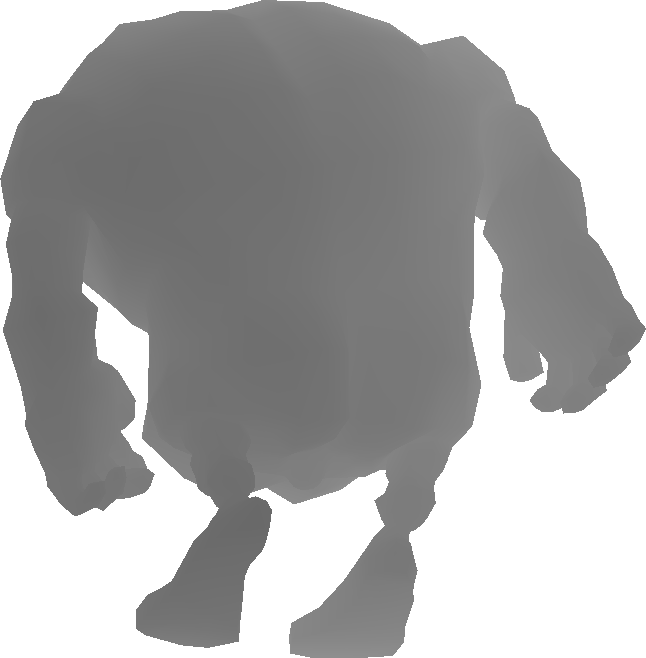
\includegraphics[width=0.4\textwidth]{\rootPath Imgs/precompute_ambiant/zbuffer.png}
	\caption{Z-buffer issu de la première étape de rendu (shadowmap)}
	\label{fig:precompute_ambiant:zbuffer}
\end{figure}


Ces données de profondeur permettent ensuite d'évaluer si un texel est visible ou non, simplement en comparant la profondeur du texel considéré et celui retenu dans la texture et qui caractérise le texel le plus proche selon le rayon associé.

La seconde étape de rendu consiste alors à écrire, dans l’espace texture associé à l'objet, les informations de visibilités qui auront été calculées (voir figure~\ref{fig:precompute_ambiant:singlesource}). À cette étape, il est important de s'assurer que la texture est bien écrite, y compris au niveau des jointures entre les différents éléments qui peuvent demander un ajustement.\cite{Aila2005}\cite{Manson2012}

\begin{figure}[!ht]\centering
	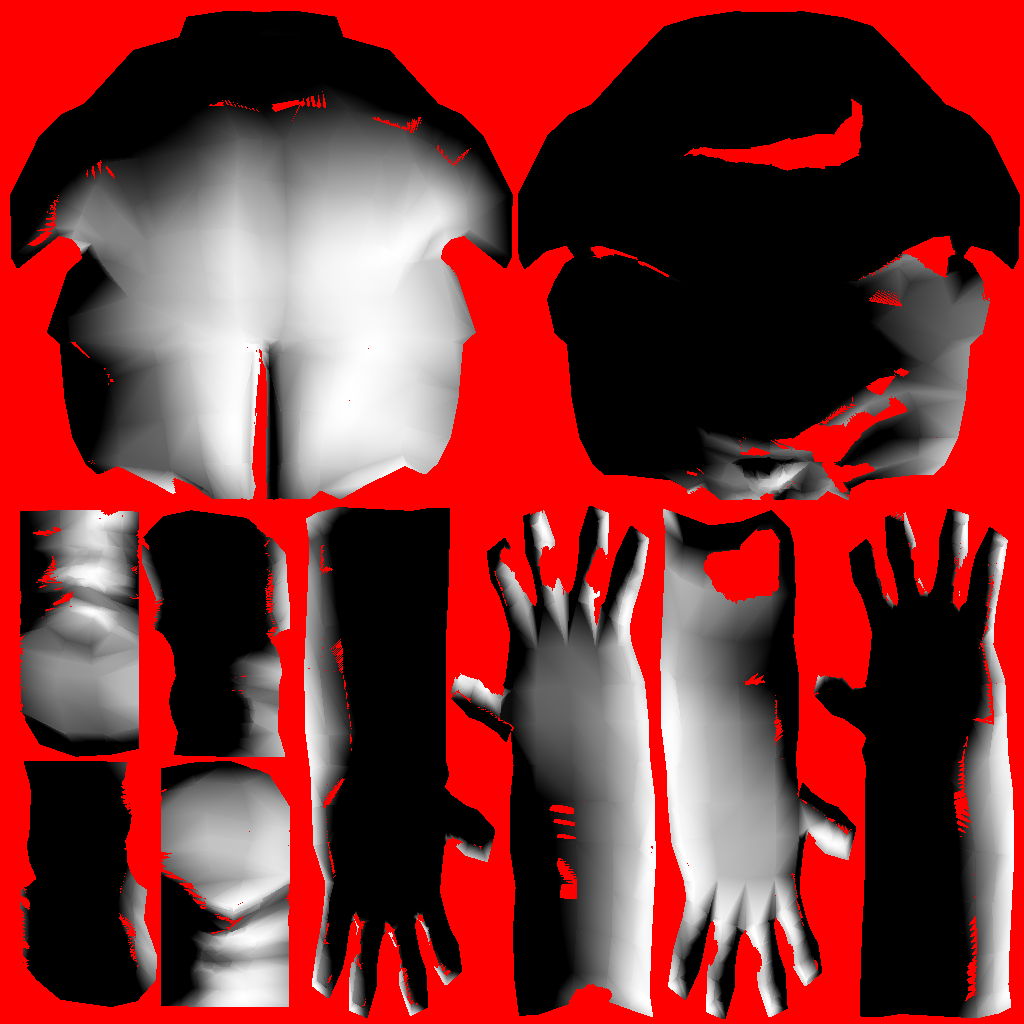
\includegraphics[width=0.4\textwidth]{\rootPath Imgs/precompute_ambiant/singlesource_red.png}
	\caption{Rendu en espace texture pour une source}
	\label{fig:precompute_ambiant:singlesource}
\end{figure}

\subsection{Post-traitement}
Une fois évalués pour une source, les résultats sont ajoutés à une texture qui somme les contributions des différentes sources. Cette texture contient ainsi le résultat de l'intégration considérée.

Une fois toutes les sources évaluées, il reste quelques étapes de post-traitement :
\begin{itemize}
	\item L'intégration étant normalisée, les valeurs calculées sont théoriquement entre $0.0$ et $1.0$. Cependant du fait de la distribution aléatoire des sources utilisées pour l'intégration, il peut arriver qu'en certains points ne pressentant pas d'auto-occultation la valeur dépasse $1.0$. Les valeurs sont alors seuillées afin de ne pas poser de problèmes au moment du stockage au format \texttt{.png}.

	Les données étant quantifiées entre $0$ et $255$, un dépassement de la valeur flottante à stocker peut provoquer une traduction en un entier supérieur à $255$. Ces nombres étant stockés sous forme de caractères ASCII, un dépassement à $256$ ou $257$ peut alors provoquer une évaluation modulo $256$ soit un stockage sous forme de $0$ ou de $1$.

	\item Les parties de l'image ne correspondant pas à des coordonnées de textures valides étant jusque-là vides. L'évaluation des niveaux de mipmap pour la texture considérée risque de prendre en compte des éléments qui ne sont par représentatifs de la réalité géométrique de l'objet. Afin de limiter ce biais dans l'évaluation des niveaux de mipmap, on remplit les parties vides et non représentative avec la valeur moyenne calculée sur les parties représentatives. Ainsi on limite l’incohérence des données considérées en bordure de patch pour les niveaux de mipmap les plus élevés.
\end{itemize}

A l'issue de ces différents post-traitement, il ne reste qu'à exporter la texture sous forme d'image (voir figure~\ref{fig:precompute_ambiant:postprocess}) qui sera chargée le moment voulu.

\begin{figure}[!ht]\centering
	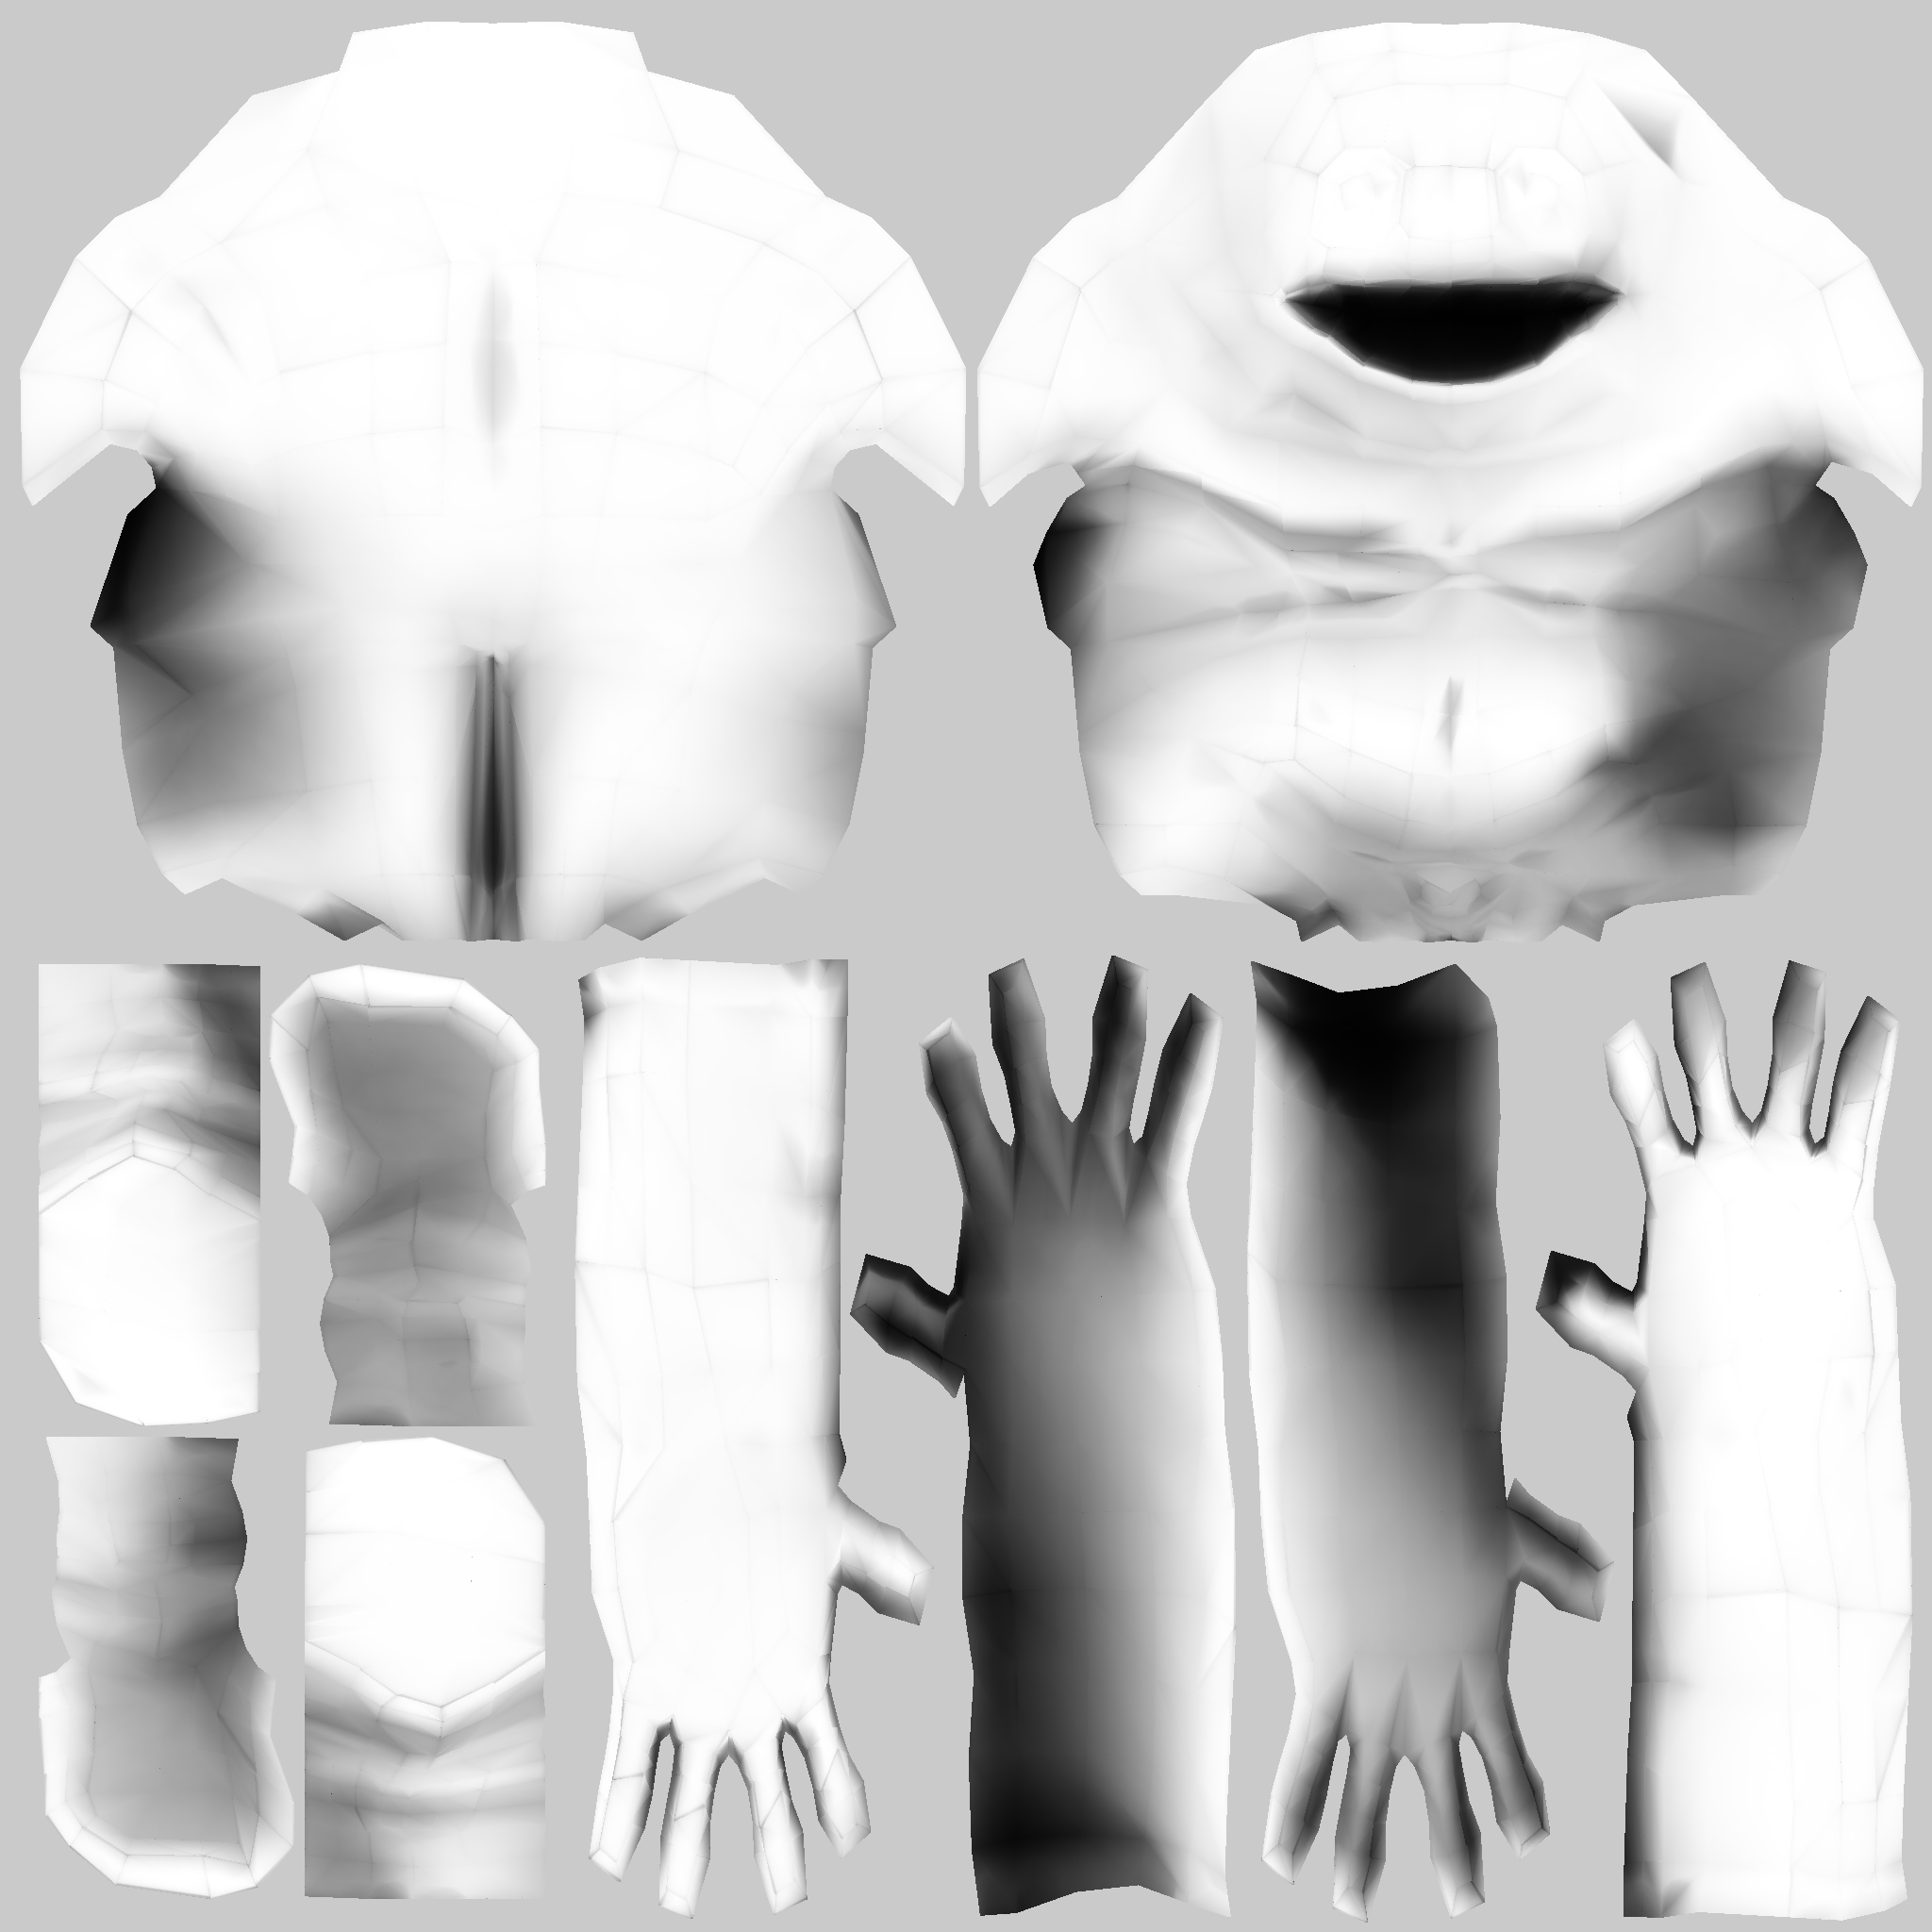
\includegraphics[width=0.4\textwidth]{\rootPath Imgs/precompute_ambiant/postprocess.png}
	\caption{Données pré-calculées en espace texture après post-traitement (1000 sources)}
	\label{fig:precompute_ambiant:postprocess}
\end{figure}

\begin{figure}[!ht]\centering
	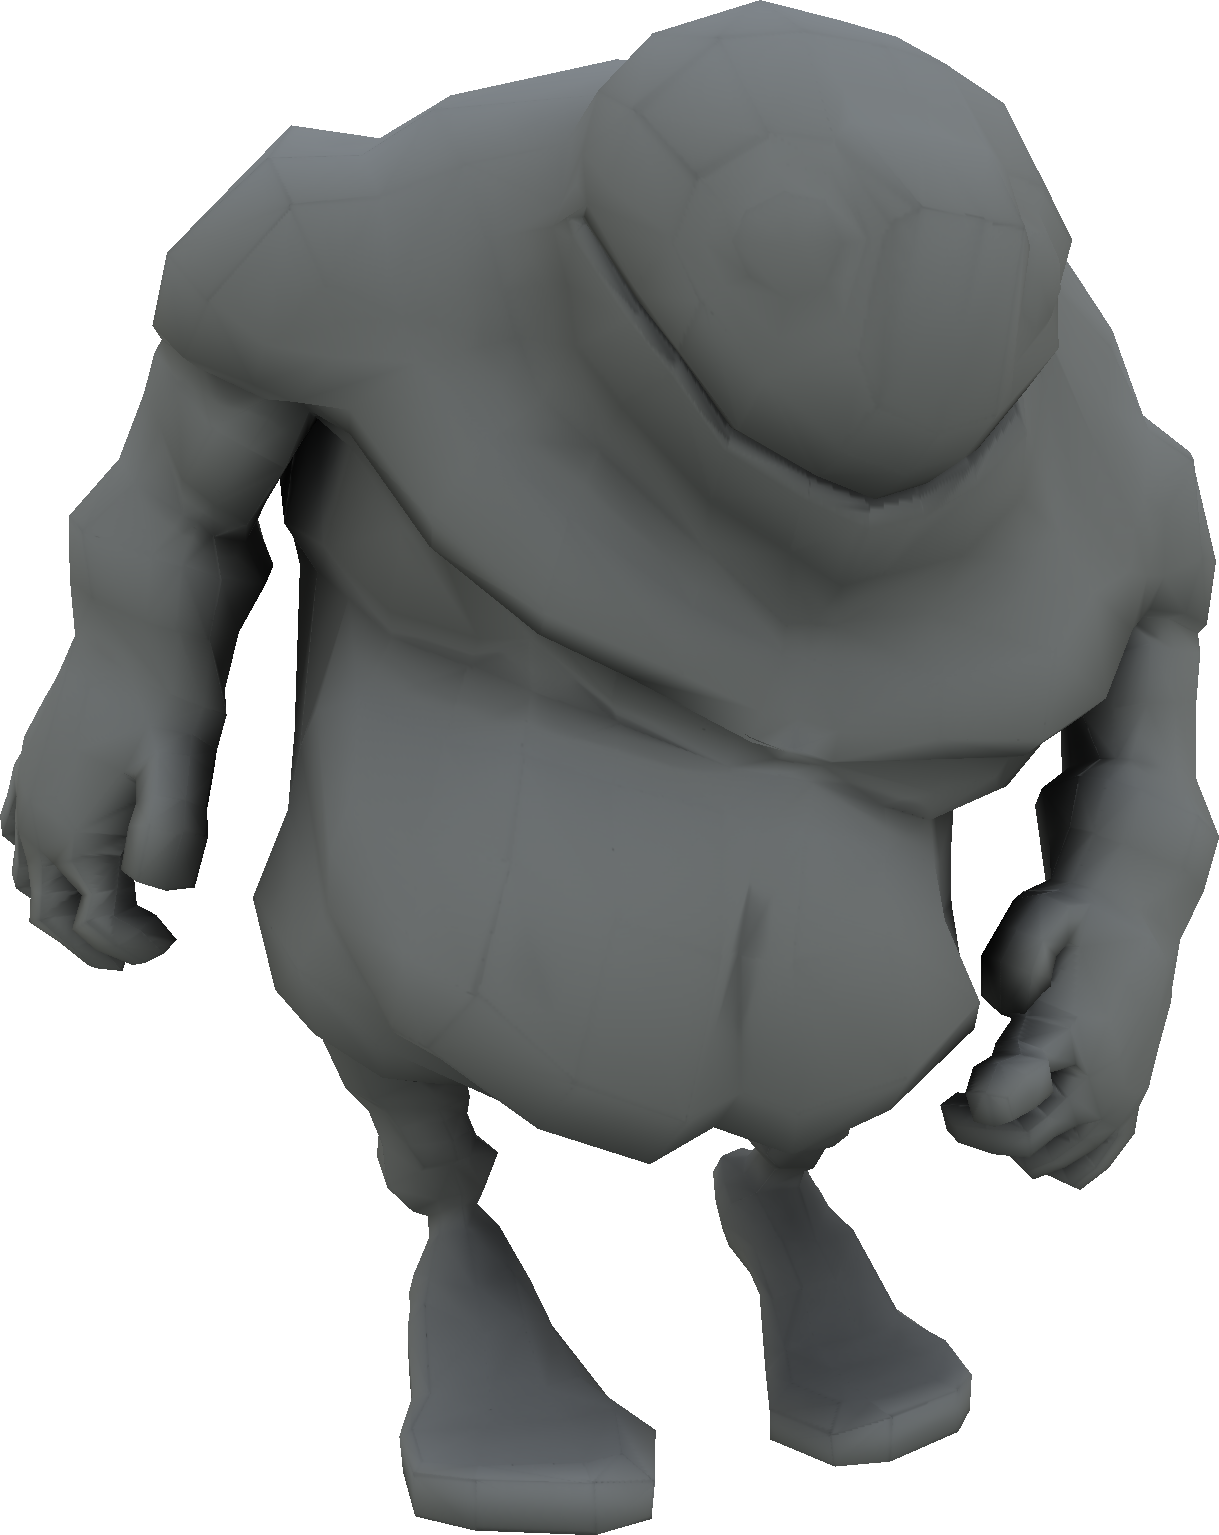
\includegraphics[height=4cm]{\rootPath Imgs/precompute_ambiant/view3.png}
	\hspace{0.5cm}
	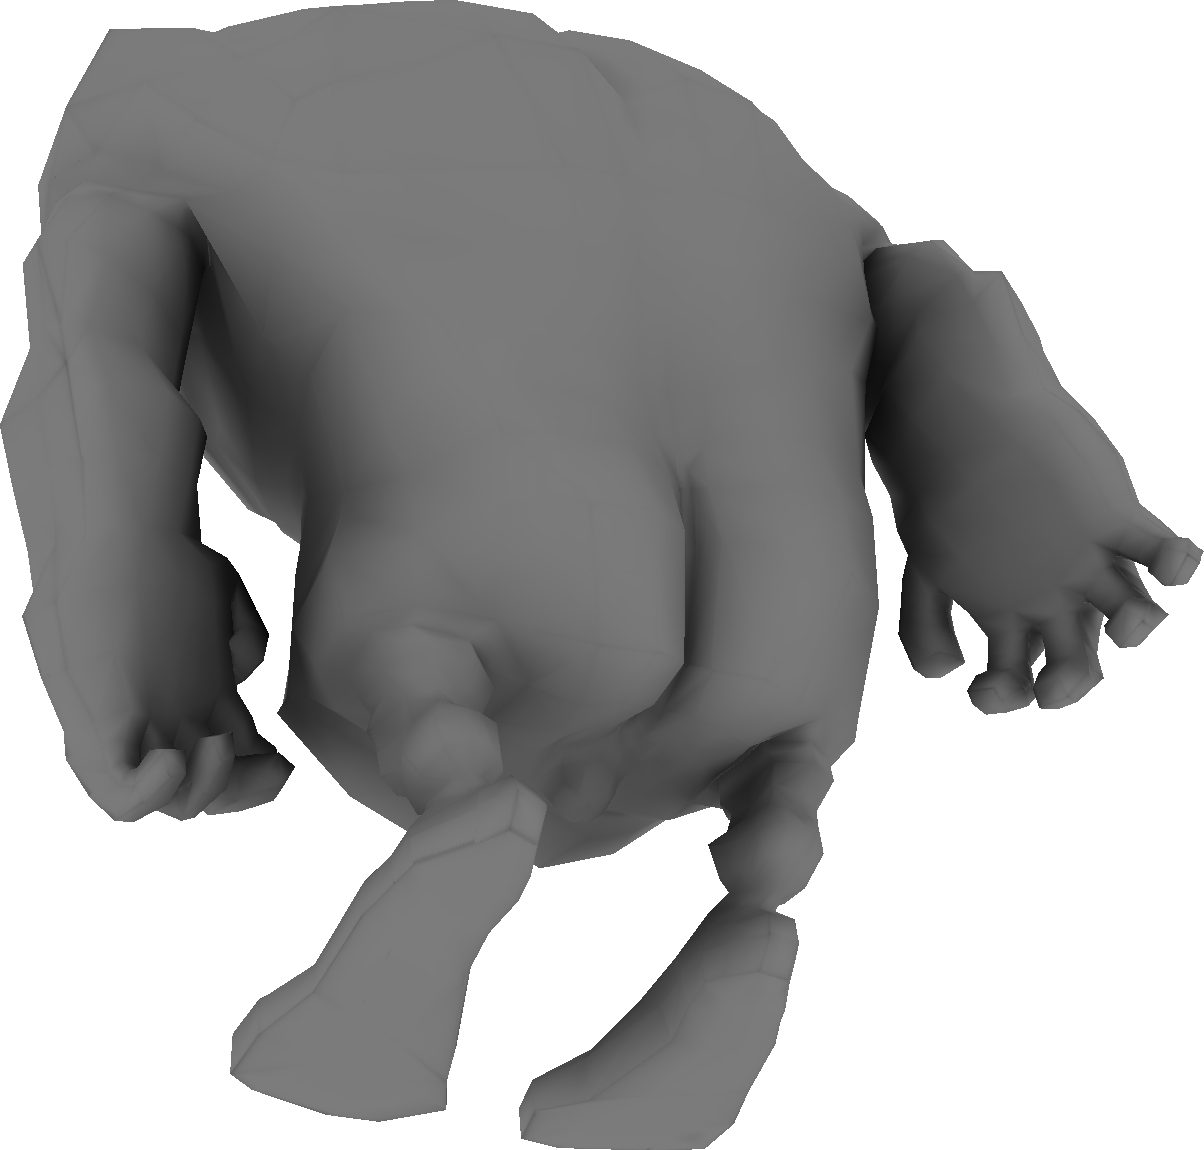
\includegraphics[height=4cm]{\rootPath Imgs/precompute_ambiant/view2.png}
	\caption{Utilisation des données d'éclairage ambiant lors du rendu}
	\label{fig:precompute_ambiant:view}
\end{figure}



\section{Décomposition en sphères}\label{section:precomputation_spheres}
La section~\ref{section:ombres}, page~\pageref{section:ombres}, traite du rendu d'ombres portées issues de l'objet 3D ajouté à la scène. Cette étape nécessite une représentation de l'objet en question comme union de sphères.

Le pré-calcul étudié ici consiste donc à construire, étant donné un maillage, un ensemble limites de sphères qui s'approche au mieux de la surface correspondant au maillage.

Ce problème d'optimisation est longuement développé dans la littérature\cite{Marshall1997}\cite{Gross2003}, notamment pour la reconstruction de surfaces implicites à partir de points (orientées ou non). La plupart des méthodes consistent à ajuster des surfaces contraintes à l'aide d'outils statistiques. Ces méthodes présentent cependant le défaut d’être mathématiquement complexes et numériquement complexes.

Le choix s'est donc porté sur une méthode simple et inexacte mais suffisante au regard de l'utilisation des résultats par l'algorithme de calcul des ombrages.

\begin{algorithm}[ht]
	\SetKwData{Mesh}{Maillage}
	\SetKwData{Point}{Point}
	\SetKwData{Sphere}{Sphere}
	\SetKwData{int}{int}
	\SetKwFunction{UniformSample}{EchantionnageUniforme}
	\SetKwFunction{Clustering}{Appareillement}
	\SetKwFunction{BestMatchingSphere}{SphereOptimale}

	\Entree{\Mesh $m$, \int $n$, \int $s$}
	\BlankLine
	\tcc{Échantillonnage du maillage}
	\Point $pts[s]$\;
	\Pour{$i \leftarrow [1..s]$}{
		$pts[i] \leftarrow \UniformSample(m)$\;
	}
	\BlankLine
	\tcc{Initialisation des sphères}
	\Pour{$i \leftarrow [1..n]$}{
		$sphs[i] \leftarrow pts[i]$\;
	}
	\BlankLine
	\Tq{$sphs$ n'est pas stable}{
		\Point $clsts[n][]$\;
		\Pour{$i \leftarrow [1..n]$}{
			$clsts[i] \leftarrow \Clustering(pts, sphs[i])$\;
		}
		\Pour{$i \leftarrow [1..n]$}{
			$sphs[i] \leftarrow \BestMatchingSphere(clsts[i])$\;
		}
	}
	\Retour{$sphs$}\;
	\caption{Ajustement de sphères à un maillage}
\end{algorithm}

\subsection{Échantillonnage du maillage}

Afin d'obtenir une distribution uniforme de points à la surface de l'objet, on procède à un échantillonnage par importance\footnote{Importance sampling}.

Pour construire un point uniformément à la surface du maillage, on sélectionne d'abord une face proportionnellement à sa surface avant de choisir un point uniformément sur la face considéré.

En répétant cette opération un grand nombre de fois on obtient un nuage de points qui représente correctement les grandes faces. Ce sont ces points qui seront utilisés par la suite pour la construction des sphères représentatives.

\subsection{Appareillement de points et calcul de sphères optimales}

La phase d'appareillement de l'algorithme consiste à organiser les points en clusters relatifs aux sphères déjà construites. Il s’agit donc d’établir une métrique qui caractérise la proximité d'un point à une sphère. De la même manière, la phase de calcul de sphères optimales consiste à calculer la sphère qui minimisera la métrique considère précédemment sur le cluster qui lui a été associé.

La principale difficulté ici est de construire un métrique représentative des critères de qualités voulus, pour laquelle le calcul d'un élément optimal n'est pas trop complexe et qui converge vers un état stable.

\subsubsection{Première approche}

Une métrique envisagéz est d'évaluer la distance d'un point à la surface de la sphère associé :
\begin{align}
	f(P, S) &= \left\|P-S\right\|^2 - S.r^2															\label{eq:metrique}	\\
					&= (P.x-S.x)^2 + (P.y-S.y)^2 + (P.z-S.z)^2 - S.r^2					\notag \\
					&= (P.x^2 + P.y^2+P.z^2) + (S.x^2+S.y^2+S.z^2)							\notag \\
					&\quad - 2(P.xS.x + P.yS.y + P.zS.z)  - S.r^2								\notag \\
					&= \|P\|^2 + \|S\|^2 - 2(P.xS.x + P.yS.y + P.zS.z) - S.r^2	\notag
\end{align}

Ce calcul de la sphère optimal associé a un cluster peut ensuite se faire par l'optimisation d'un système matriciel $AX-B$, la matrice $A$ représentant les données en entrée (points échantillonnées), le vecteur $X$ représentant la solution à optimiser et le vecteur $B$ étant l'objectif à atteindre.

L'équation~\ref{eq:metrique} nous indique comment construire $A$, $X$ et $B$ :
\begin{subequations}
\begin{align}
		A	&=	\begin{pmatrix}
						-2P_1.x & -2P_1.y & -2P_1.z & 1 			\\
						-2P_2.x & -2P_2.y & -2P_2.z & 1 			\\
						\vdots	& \vdots	&	\vdots	& \vdots	\\
						-2P_n.x & -2P_n.y & -2P_n.z & 1
					\end{pmatrix}																												\\
		X &=	\begin{pmatrix} S.x \\ S.y \\ S.z \\ \|S\|^2 - S.r^2 \end{pmatrix}	\\
		B	&=	\begin{pmatrix}
						\|P_1\|^2	\\
						\|P_2\|^2	\\
						\vdots			\\
						\|P_n\|^2
					\end{pmatrix}																												\\
\intertext{Ainsi on a :}
	A.X+B &= \begin{pmatrix}
						f(P_1, S)	\\
						f(P_2, S)	\\
						\vdots		\\
						f(P_n, S)
					\end{pmatrix}
\end{align}
\end{subequations}

Cette première considération géométrique n'est cependant pas satisfaisante. La simple proximité entre un point et la surface d'une sphère ne prend pas en compte les différences d'orientation de normale entre une face du maillage et la sphère qui le modélise, lesquels sont des éléments de qualité essentiels dans notre cas. Au delà de ce problème d'orientation, cette métrique fait aussi face au problème des outliers présents sur les modèles non convexes. Si quatre points extrémaux se retrouvent loin de tout, il est possible qu'une sphère viennent les adopter comme point d'attache, englobant alors tout le modèle et cachant la géométrie que l'on voulais représenter.

Par ailleurs la métrique proposé précédemment ne garanti pas la convergence du système.

\begin{figure*}[!ht]\centering
	\begin{subfigure}[b]{\textwidth}\centering
		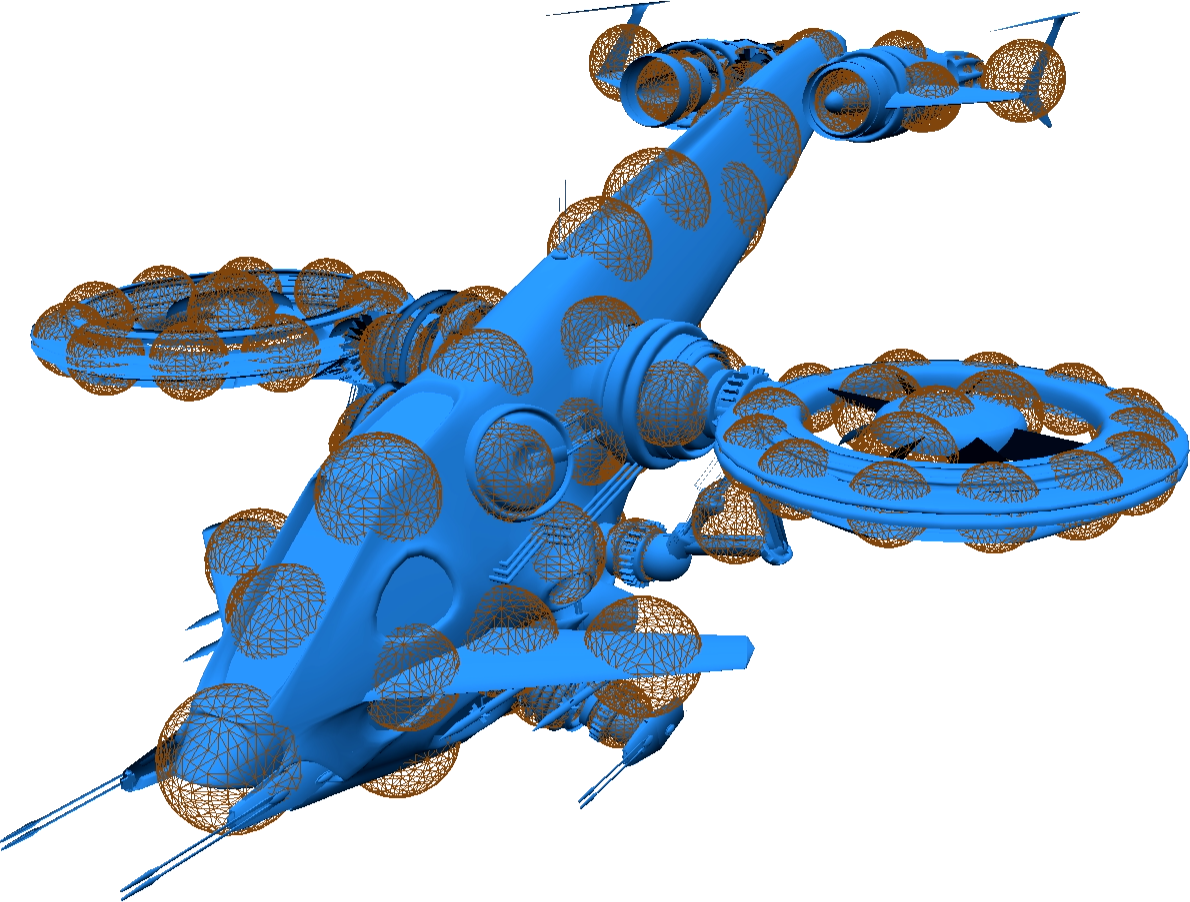
\includegraphics[width=0.4\textwidth]{\rootPath Imgs/precompute_spheres/MRX22_both.png}
		\vspace{0.5cm}
		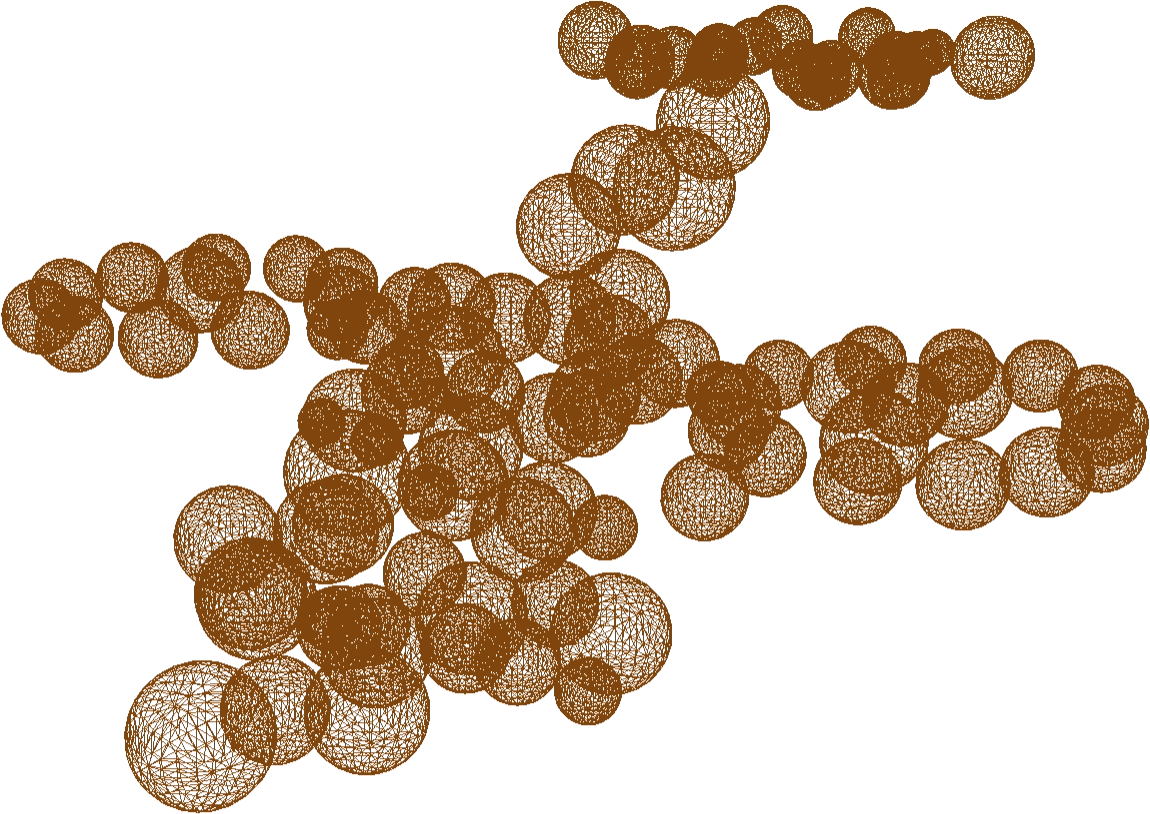
\includegraphics[width=0.4\textwidth]{\rootPath Imgs/precompute_spheres/MRX22_spheres.png}
		\caption{MRX22 (157781 sommets, 287776 triangles)}
	\end{subfigure}

	\begin{subfigure}[b]{\textwidth}\centering
		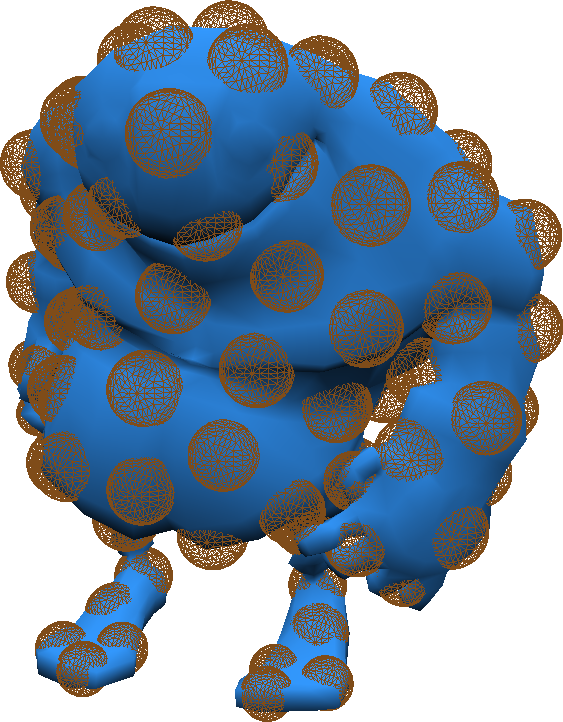
\includegraphics[width=0.4\textwidth]{\rootPath Imgs/precompute_spheres/bigguy_both.png}
		\vspace{0.5cm}
		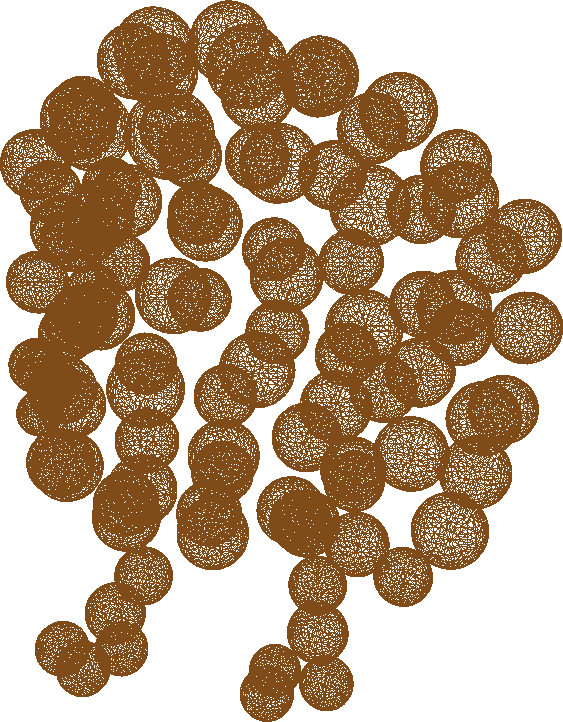
\includegraphics[width=0.4\textwidth]{\rootPath Imgs/precompute_spheres/bigguy_spheres.png}
		\caption{Bigguy (1754 sommets, 2900 triangles)}
	\end{subfigure}
	
	\caption{Décomposition en sphères d'objets 3D ($100000$ échantillons, $100$ sphères)}
	\label{fig:precompute_sphere:result}
\end{figure*}

\subsubsection{Méthode adoptée}

Finalement la solution adoptée, bien que géométriquement pauvre, nous donne des résultats visuellement acceptables tout en garantissant une convergence rapide. L'idée est de paver la surface du maillage à l'aide de sphères de rayon uniforme, ce qui correspond à la minimisation de la distance entre les points et le centre des sphère qui leur sont associés (voir figure~\ref{fig:precompute_sphere:result}).

La distance considérée
\begin{align}
	f(P, S)			&= \left\|P-S\right\|	\\
\intertext{s'optimisant trivialement sur un cluster $C$ par}
	\overline S	&= \left\{ \left(\overline p, \overline{\|p-s\|}\right)\;|\;p \in C \right\}
\end{align}

%=====================================================================
%=====================================================================
\ifstandalone
	\addcontentsline{toc}{chapter}{Bibliographie}
	\bibliographystyle{apalike}
	\bibliography{\rootPath Annexes/biblio}
\fi
%=====================================================================
%=====================================================================
\end{document}